\section{Classification using the amplitude only}

Eine Klassifikation anhand von x1 alleine wird nur sehr schlecht funktionieren, da in 
x1 auf den ersten Blick relativ wenig information über die Klassenzugehörigkeit steckt.
Bei der Kombination aus x1 und x2 kann man sich also eine deutlich bessere Klassifikationsperformance erwarten.


\begin{figure}[ht!]
 \centering
 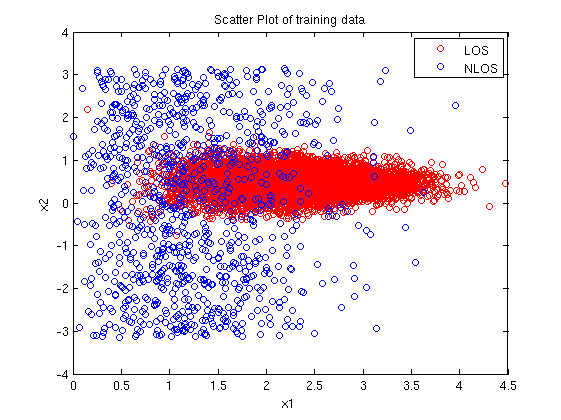
\includegraphics[bb=0 0 449 336]{./figures/5_1_1_trainingdata.png}
 % 5_1_1_trainingdata.png: 561x420 pixel, 90dpi, 15.83x11.85 cm, bb=0 0 449 336
 \caption{Trainingsdatensatz}
 \label{abb:trainingdata}
\end{figure}

\begin{enumerate}
 \item 

\begin{equation}
 p(x_1|t=NLOS) = \frac{x_1}{\sigma^2} exp(\frac{-x^2}{2\sigma^2})
\end{equation}
\begin{equation}
 log(p(x_1^1, ..., x_1^N| \sigma)) = log \prod_{n=1}^N p(x_1^n|NLOS) = \sum_{n=1}^N log(\frac{x_1}{\sigma^2} exp(\frac{-x^2}{2\sigma^2}))
\end{equation}

\begin{equation}
\frac{\partial}{\partial \sigma} = \frac{-2N}{\sigma} + \sigma^{-3} \cdot \sum_{n=1}^N (x_1^n)^2 = 0
\end{equation}
\begin{equation}
 \sigma = \sqrt{\frac{\sum_{n=1}^N (x_1^n)^2}{2N}}
\end{equation}


\item -
\item Die Normalisierung erfolgt durch Multiplizieren jedes Balkens des Histogramms mit dem folgenden Normalisierungsfaktor:
\begin{equation}
 \frac{\#Balken}{(\sum N) * X(end) - X(1)}
\end{equation}
Wobei N die Balkenhöhe und X der zugehörige Balkenmittelpunkt auf der X-Achse darstellt
\item 
ML-Klassifikation: Es wurden 85.1455\% korrekt klassifiziert \\
Bayes-Klassifikation: Es wurden 93.8364\% korrekt klassifiziert \\
Mittels der Bayes Klassifikation lässt sich aufgrund der Priorwahrscheinlichkeit ein besseres Ergebnis erzielen.
Die gute Klassifikationsperformance beruht aber eigentlich nur darauf, dass die meisten Daten LOS sind und nur
wenige NLOS sind. Währe die Priorwahrscheinlichkeit für NLOS und LOS gleich, würde man deutlich schlechtere Ergebnise
erzielen.
\item




\end{enumerate}

\begin{figure}[ht!]
 \centering
 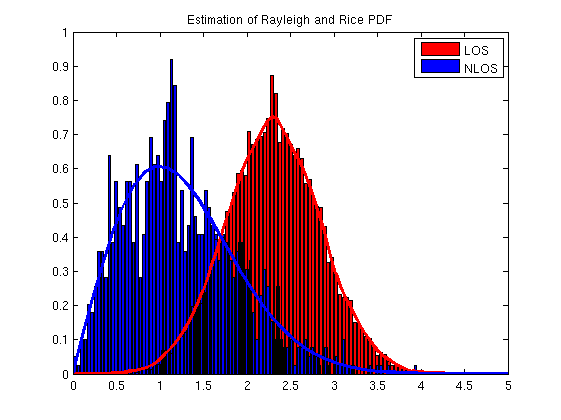
\includegraphics{./figures/5_1_1_estimation.png}
 % 5_1_1_trainingdata.png: 561x420 pixel, 90dpi, 15.83x11.85 cm, bb=0 0 449 336
 \caption{Estimation of PDF-Parameters}
 \label{abb:estimation}
\end{figure}


\begin{figure}[ht!]
 \centering
 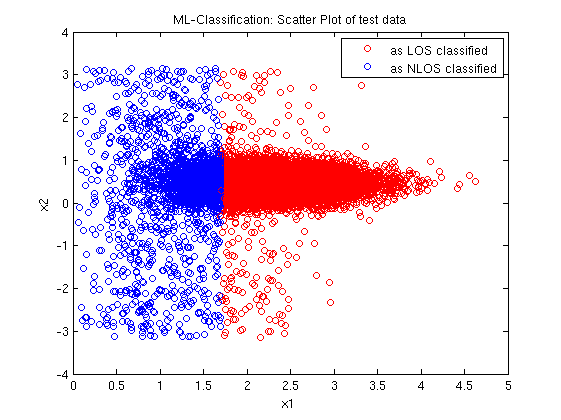
\includegraphics{./figures/5_1_1_ml.png}
 % 5_1_1_trainingdata.png: 561x420 pixel, 90dpi, 15.83x11.85 cm, bb=0 0 449 336
 \caption{ML-Klassifikation}
 \label{abb:ml}
\end{figure}

\begin{figure}[ht!]
 \centering
 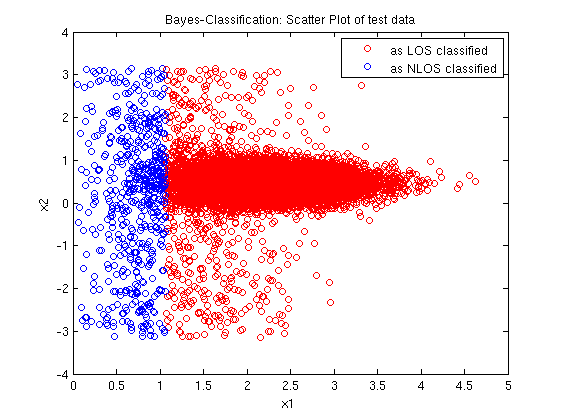
\includegraphics{./figures/5_1_1_bayes.png}
 % 5_1_1_trainingdata.png: 561x420 pixel, 90dpi, 15.83x11.85 cm, bb=0 0 449 336
 \caption{ML-Klassifikation}
 \label{abb:bayes}
\end{figure}
